% ______________________________________________________________________________
%
%   2DV513 Database Theory -- Assignment 1
%
%   Author:  Jonas Sjöberg
%            Linnaeus University
%            js224eh@student.lnu.se
%            github.com/jonasjberg
%            www.jonasjberg.com
%
%  License:  Creative Commons Attribution 4.0 International (CC BY 4.0)
%            <http://creativecommons.org/licenses/by/4.0/legalcode>
%            See LICENSE.md for additional licensing information.
% ______________________________________________________________________________


\section{Task 4 --- Classroom Scheduling}
Exercise from \emph{Database System Concepts, 5th Edition} \cite{2dv513:dsc},
section 6.6.

\subsection{Problem Description}
The problem description \cite{2dv513:assignment1-instructions} is stated as
follows:

\begin{quote}
  Consider a university database for the scheduling of classrooms for the final
  exams.

  This database could be modeled as a single entity set \emph{exam} with
  attributes
  \emph{course\_name}, \emph{section\_number}, \emph{room\_number},
  and \emph{time}.

  Alternatively, one or more additional entity sets could be defined, along
  with relationship sets to replace some of the attributes of the \emph{exam}
  entity set, as:

  \begin{enumerate}
    \item
      \emph{course} with attributes \emph{name}, \emph{department},
      and \emph{c\_number}.

    \item
      \emph{section} with attributes \emph{s\_number} and \emph{enrollment},
      and dependent as a weak entity set on \emph{course}.

    \item
      \emph{room} with attributes r\_number}, capacity, and building.
  \end{enumerate}

  Show an E/R diagram illustrating the use of all three additional entity sets
  listed.

  Explain what application characteristics would influence a decision to
  include or not include each of the additional entity sets.

  \emph{Note:} A section is a part of course. How sections are used varies from
  university to university, but they could for example be used to separate
  multiple versions of the course (imaging that a course has so many students
  that there has to be parallel lectures) or if a course is given multiple
  times per year.
\end{quote}


\subsection{Solution}
The proposed solution is shown in Figure~\ref{fig:task4}.

\begin{figure}[htbp]
  \centering
  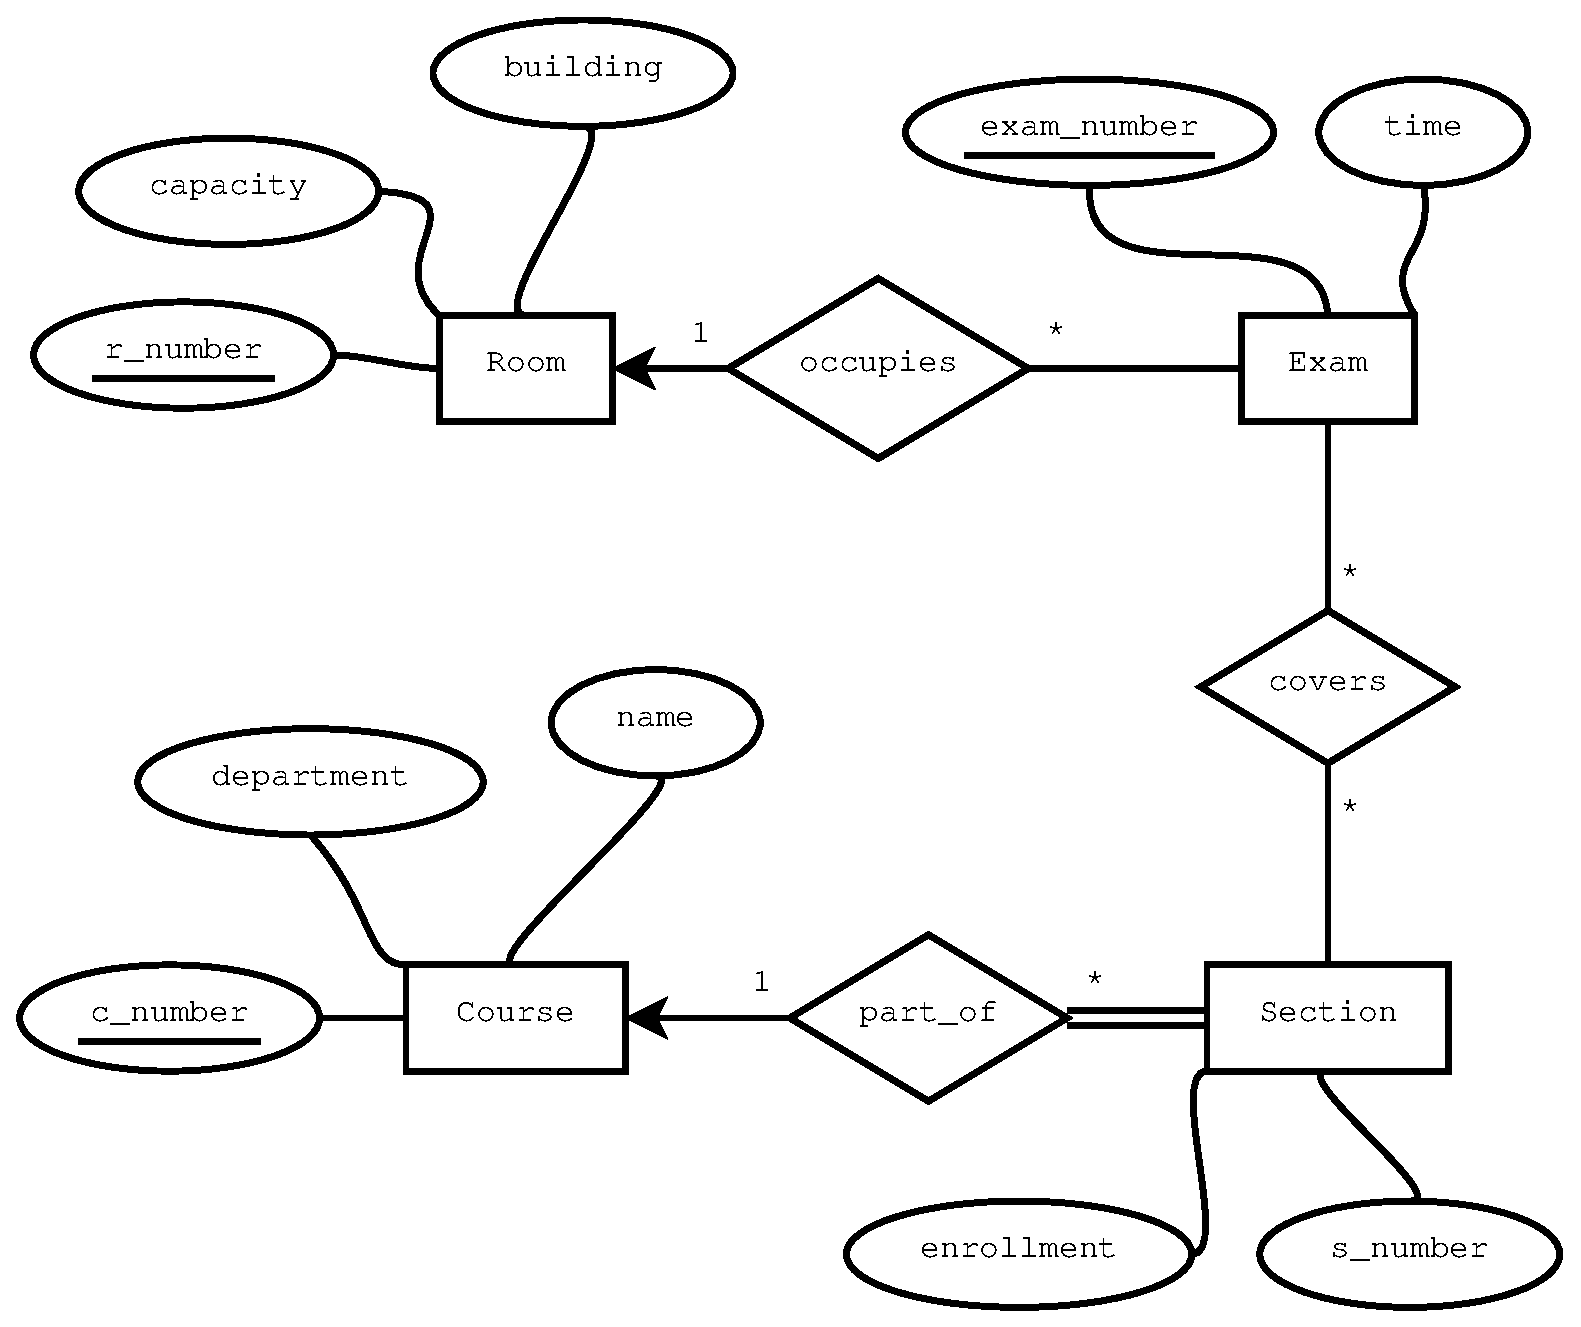
\includegraphics[width=\linewidth]{include/task4.eps}
    \caption{Entity-relationship Diagram for Task 4}
  \label{fig:task3}
\end{figure}

Some of the original attributes have been bundled into new entities. The
original attributes that contained a underline and a shared prefix was
extracted into a new entity. The common prefix became the entity name. This
change seemed very similar to refactoring techniques I frequently use when
writing software.

The new entities were then linked using the most basic relations, with names
borrowed from the previous task.

Broadly, applications where maintainability and adjusting the change are
likely; I.E. the schema will have to be reworked or the software application
somehow needs to query the data in some new, initially unforeseen way.

This seems analogous to structuring software; smaller, modules with well
defined responsibilities are easier to maintain and reason about than a bigger
module that handles many different tasks.

It is often desirable to modularize systems and integrate these modules using
well defined boundaries, which makes replacing modules much easier.
In this case, the scheduling database really should not be all too tangled up
with course-specific data --- a course might use a different method for
examining the students. Some courses might not have any exams at all, while
some might use a online system to do the exams.

The entities are related through the unique identifier attributes but they each
handle a distinctively different kind of data, that is open for modifications
without disrupting the other tables.
